\documentclass[a4paper]{article}
\usepackage[margin=15mm]{geometry}
\usepackage{graphicx}
\usepackage{mathpazo}
\usepackage{datetime,multicol,nicefrac}
\usepackage[colorlinks,linkcolor=blue]{hyperref}

\title{Figures and other stuff for statistics\\ using package \texttt{tikz} and \texttt{pgfplot}}
\author{Erika Griechisch}
\date{\small Last update: \today}


\begin{document}
\maketitle
\thispagestyle{empty}
	\begin{abstract}
	I teach statistics since 2014, therefore I created several exercise sheets, lecture slides for statistics teaching and besides that, sometimes I need figures when I prepare my posters. During the last few years it was a bit painful to find the best way to create figures, and to spare some time for others, hereby I include all figures in a folder I found and used from different forums (mainly on \url{http://www.texample.net/tikz/examples} and \url{https://tex.stackexchange.com/questions/tagged/tikz-pgf}). 
	

	All figures are stored in separate files using mainly \texttt{standalone} documentclass. I tried to 
	\begin{itemize}
	\item modify the original sources to make them as general as possible.;
	\item keep the original source (website) at the beginning of the file. 
		If I did not succeed and you know the original source, please let me now
	\item keep every example clear and flexible.
	
		 \texttt{TODO} comments mark the lines you have to change to adjust the figure to your data. 
	\end{itemize}

	I have to tell here I am not a pro in \LaTeX, though I use for a long time. I take examples from websites and modify them if it is necessary. If you have any idea to make the figures nicer, the sources cleaner and/or easier to understand, feel free to submit a commit or leave me a message!
	

	\end{abstract}
	
	\tableofcontents
	\clearpage
	
	\section{Form}
	
	First of all here is a form using the \texttt{paperandpencil.sty} file. 
	Finding an appropriate package to create forms or questionnaires, was really difficult. 
	I think this solution is not the best, but the best I found.
	Please let me know if you know better way of creating forms in \LaTeX{}!
	\vfill
	
	\fbox{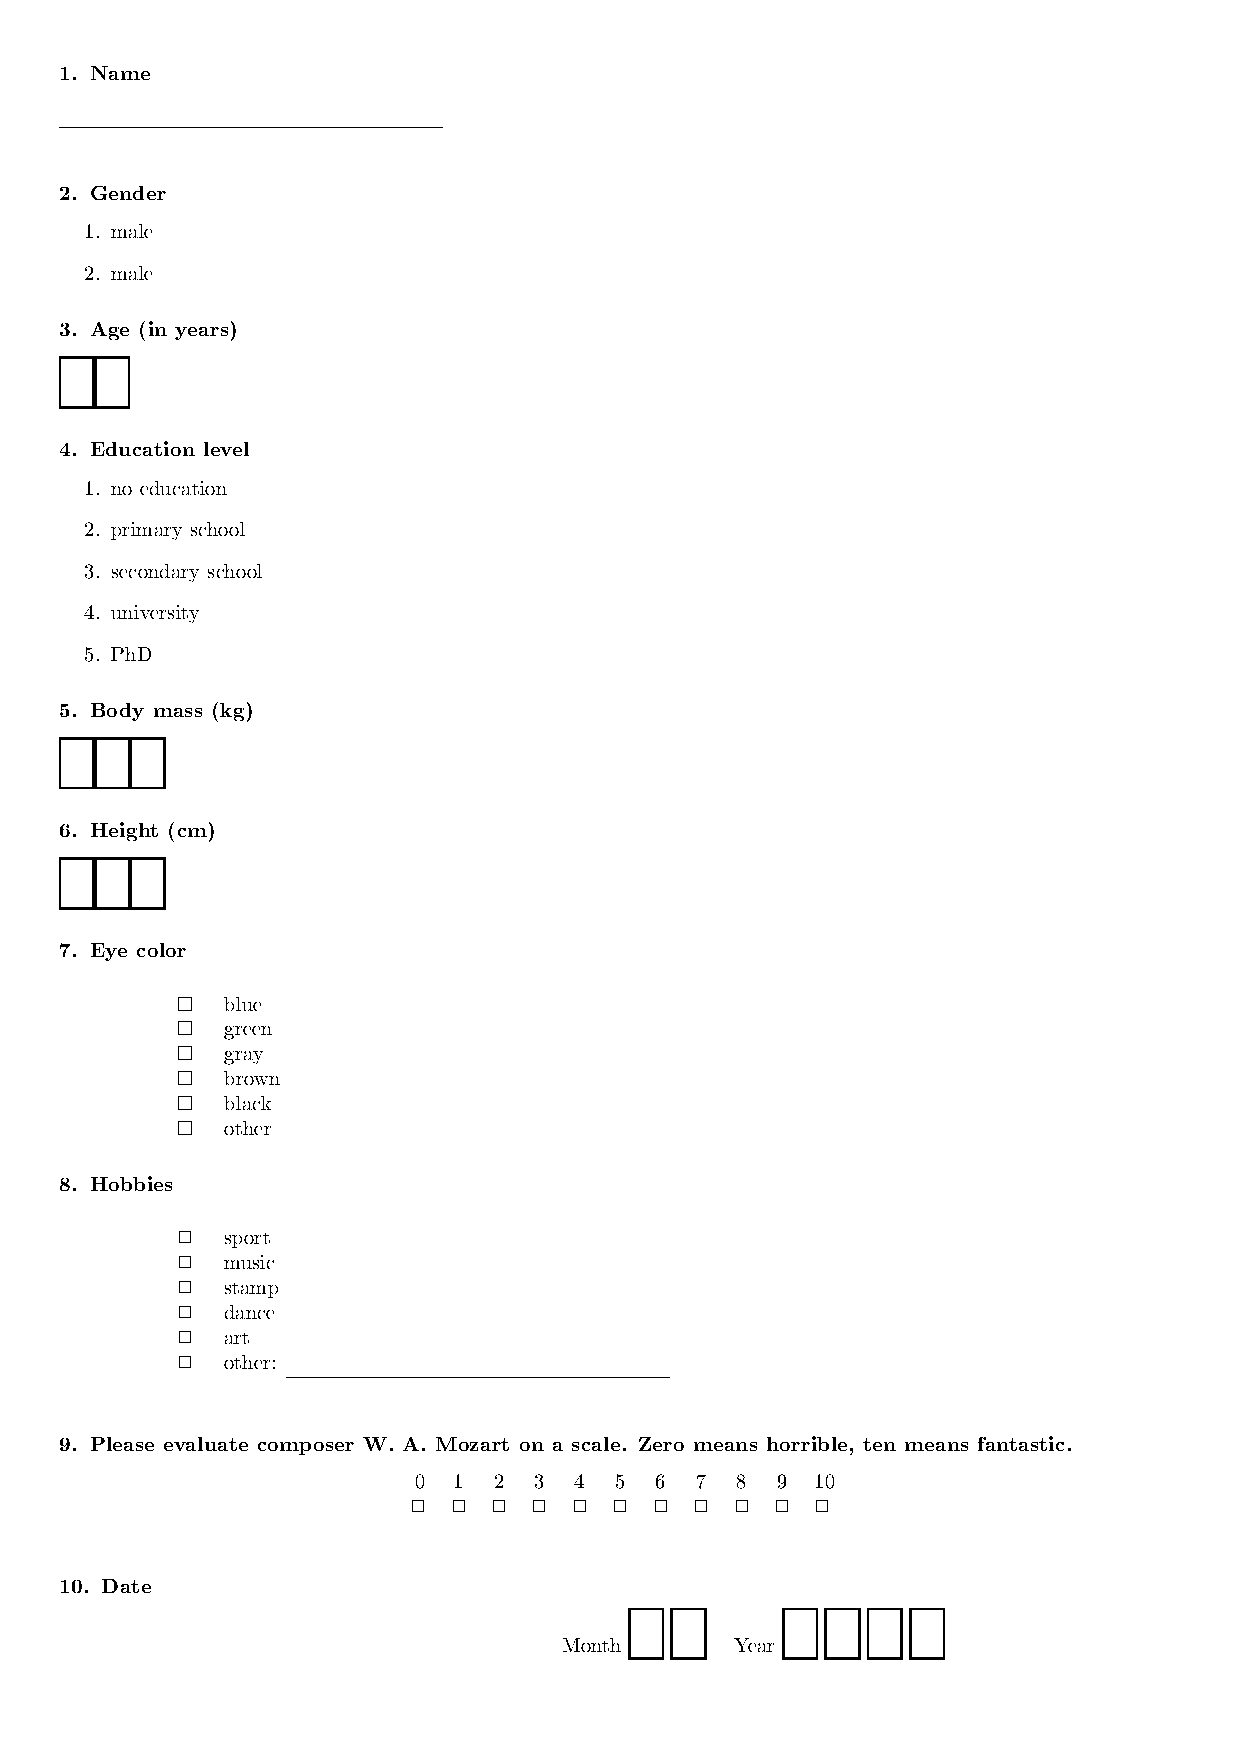
\includegraphics[width=0.95\textwidth]{form}}
	
	
	\section{Discrete variables}
	\subsection{Barplot}
	I found 2 ways of plotting barplots for two  groups. In my case I compared female and male handwriting based on the evenness of the handwriting, which has 3 possible values: even, mostly even and mixed. 
	
	The first figure one on the left is a colorful barchart. The second one is colorful as well, but includes patterns on the rectangles, so it can be used if it is uncertain whether the plot will be printed e.g. in colors or in black-and-white. 
	
	\begin{multicols}{2}	
		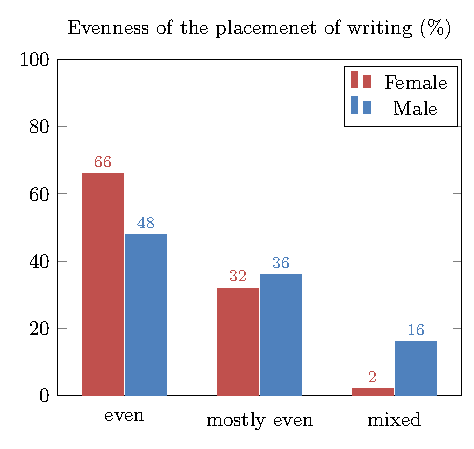
\includegraphics[width=0.45\textwidth]{barplot_with_colors}
			
		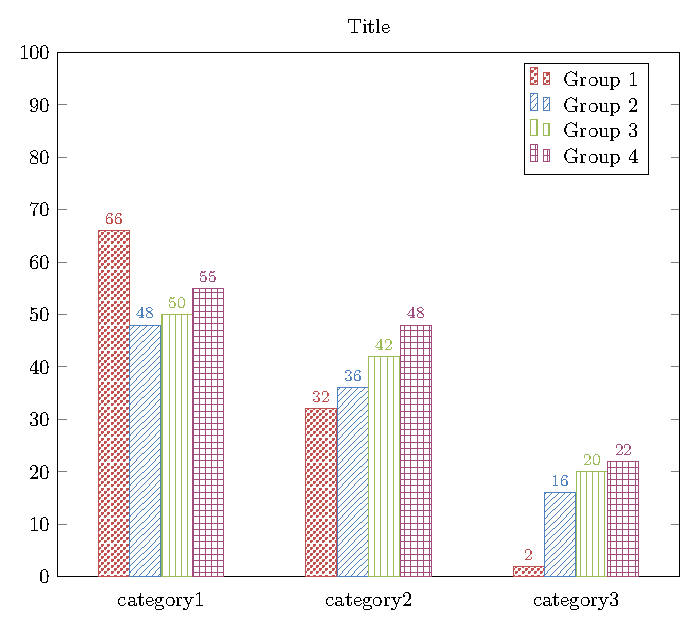
\includegraphics[width=0.45\textwidth]{barplot_with_patterns}
	\end{multicols}
	
	\subsubsection*{Change values and category}
	To show the category names below the $x$  axis, use the \verb.symbolic x coords={even,mostly even,mixed}. and change the 
	\texttt{even, mostly even, mixed} to your category names. Besides this you have to change the \texttt{addplot} line too and 
instead of using there \verb.{(even,66) (mostly even,32) (mixed,2)}. replace the category names according to the previously mentioned \texttt{symbolic x coords}. E.g. \verb.symbolic x coords={category1, category2, category3}. and \verb.{(category1,66) (category2,32) (category3,2)}..

		
	\subsubsection*{Change group names}
	\verb.\legend{Female,Male}. $\Rightarrow$ \verb.\legend{Group1, Group2}.

	
	
	\subsection{Piechart}
	I found a nice way to visualize frequencies. Check the source of the \texttt{pie1.tex} file, the original source with detailed description is given there.  It was not obviuous to me how to interpret the whole file, but it is not necessary to understand each line.
		
	\begin{center}
		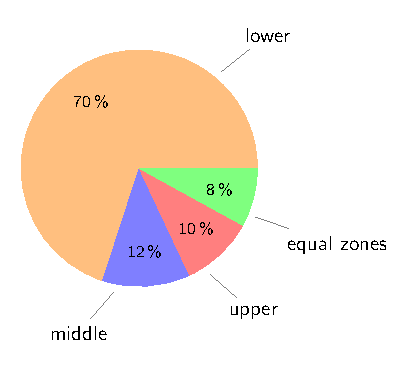
\includegraphics[width=0.4\textwidth]{pie1}
				
		%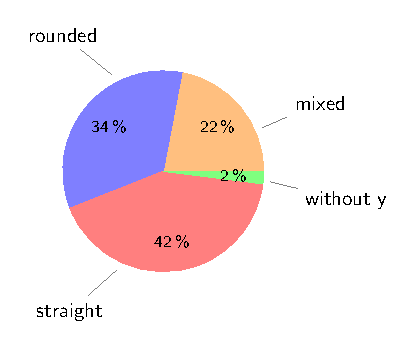
\includegraphics[width=0.4\textwidth]{pie2a}
		
		%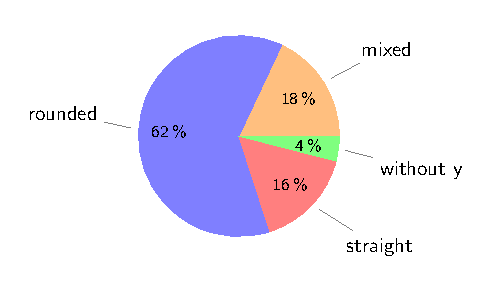
\includegraphics[width=0.45\textwidth]{pie2b}		
	\end{center}
	
	
	\subsubsection*{Change percentages and category names}
	 Find the comment starting with \texttt{TODO}, the next few lines have to be changed in order to 
	 produce piechart with different percentages.
		
	\subsubsection*{Change colors}
	The \verb.\def\cyclelist{{"orange","blue","red","green"}}. line defines the colors of the piechart. 
	
	
	\subsection{Boxplot}
	I could only find one nice way to visualise boxplots in \LaTeX{} using the \texttt{pst-plot} package. It can be compiled with \texttt{xelatex} instead of \texttt{pdflatex}. I am not really familiar with this package, but I played with the parameters I created a horizontal version of a boxplot too. If anyone would extend the sources with descriptions of the parameter in \texttt{boxplot\_vertical.tex} and \texttt{boxplot\_horizontal.tex} I would really appreciate :) Still I hope one day I will have enough time to provide a more general source.
	
	\begin{center}
		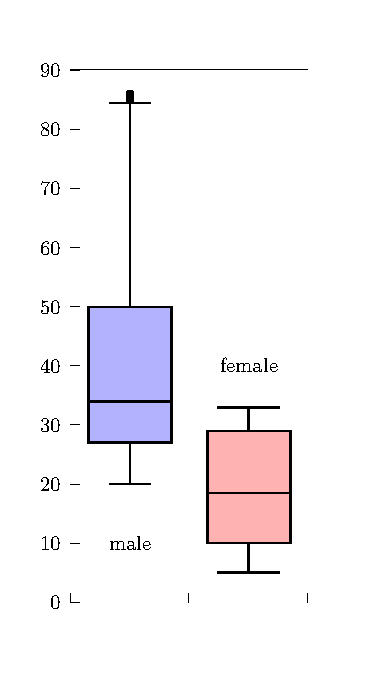
\includegraphics[width=0.4\textwidth]{boxplot_vertical}
		
		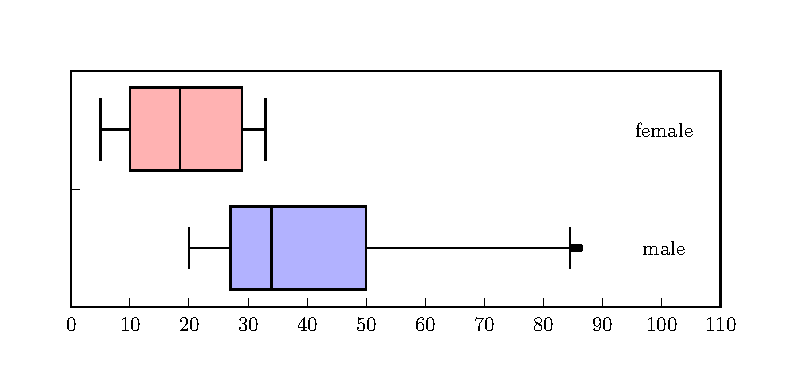
\includegraphics[width=0.8\textwidth]{boxplot_horizontal}
	\end{center}
	
	\subsection{Mean-SD diagram}
		\begin{center}
		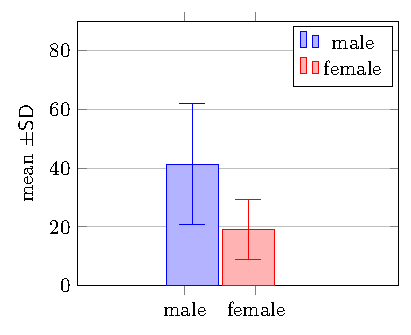
\includegraphics[width=0.5\textwidth]{mean-SD}
		
		TODO: how to enlarge the distance between the two mean-SD diagram?
	\end{center}
	
	
	\section{Discrete distributions}
	\subsection{Rolling a dice}
		\begin{multicols}{2}
			\centering
			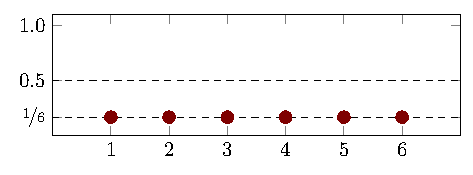
\includegraphics[width=0.5\textwidth]{Dice_single_probability}\\
			probabilities 

			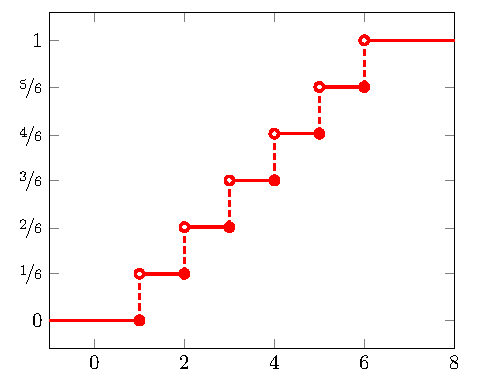
\includegraphics[width=0.5\textwidth]{Dice_single_CDF}\\
			cumulative distribution function (CDF)				
		\end{multicols}
	
	\subsection{Rolling two dices -- sum of the values}
		\begin{multicols}{2}
			\centering
			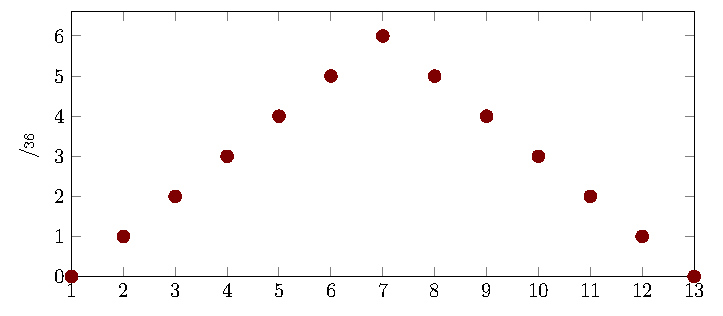
\includegraphics[width=0.5\textwidth]{Dice_double_probability}\\
			probabilities
			
			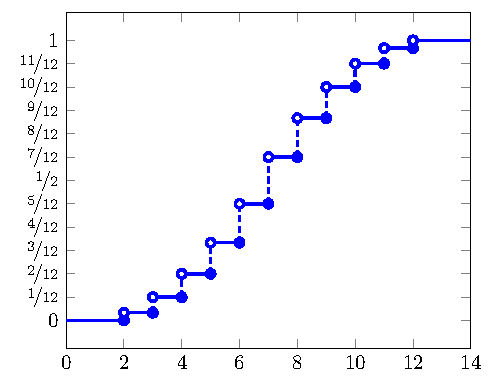
\includegraphics[width=0.5\textwidth]{Dice_double_CDF}\\
			cumulative distribution function (CDF)
		\end{multicols}


	\subsection{Tossing a coin (head or tail)?}
		\begin{multicols}{2}
		\centering
		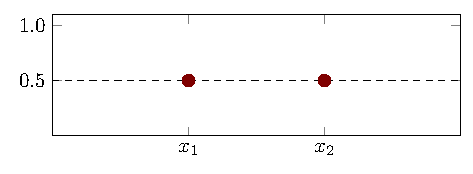
\includegraphics[width=0.5\textwidth]{tail_head_theoretical}
				
		theoretical distribution


		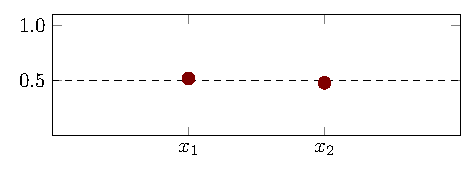
\includegraphics[width=0.5\textwidth]{tail_head_empirical}
		
		an empirical distribution\\52\% head ($x_1$), 48\% tail ($x_2$) 
		\end{multicols}
	
	
	\section{Continuous distributions}
	\subsection{Uniform  distribution}		
		\begin{multicols}{2}
		\centering
		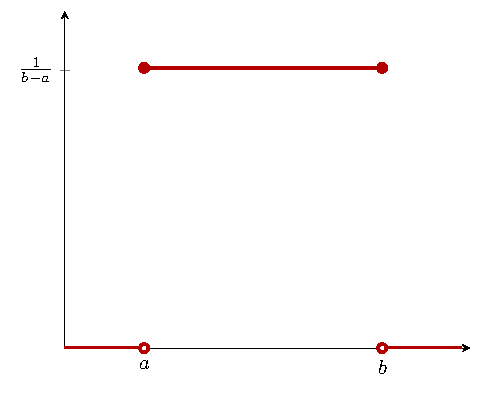
\includegraphics[width=0.5\textwidth]{uniform_density}\\
		Uniform density function\\TODO how to change the value at $a$ to 0 instead of $\nicefrac{1}{b-a}$?
		\columnbreak
		
		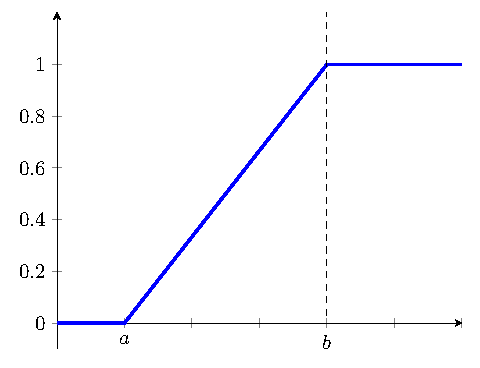
\includegraphics[width=0.5\textwidth]{uniform_distribution_CDF}\\
		Uniform cumulative distribution function
		\end{multicols}
		
	\subsection{Binomial distribution}
		\begin{multicols}{2}
		\centering
		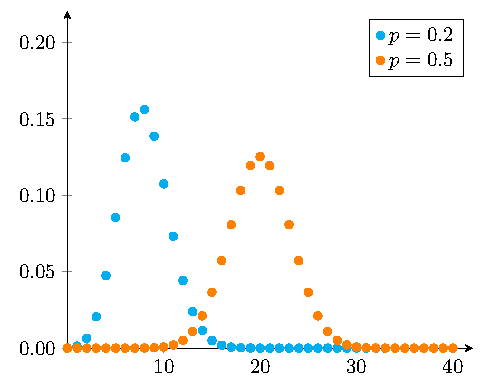
\includegraphics[width=0.5\textwidth]{Binomial-distribution}		
		
		Binomial distribution with 10 repetition ($n=10$)\\ and different $p$ values
		\columnbreak
				
		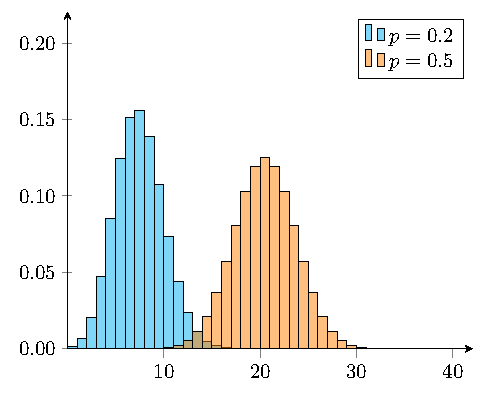
\includegraphics[width=0.5\textwidth]{Binomial-distribution-histogram}		
				
		The previous using histogram
		\end{multicols}
	
	\clearpage


	\subsection{Normal distribution}
		\begin{multicols}{2}
		\centering
		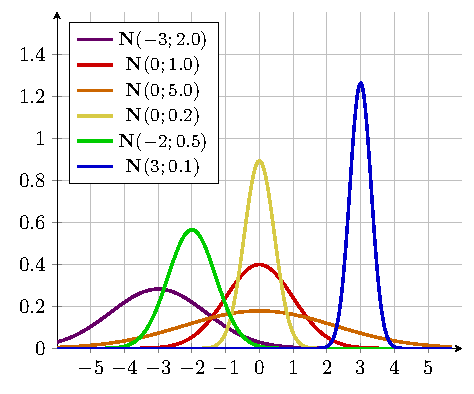
\includegraphics[width=0.5\textwidth]{normal_distributions}\\
		Normal distribution with different parameters
				
		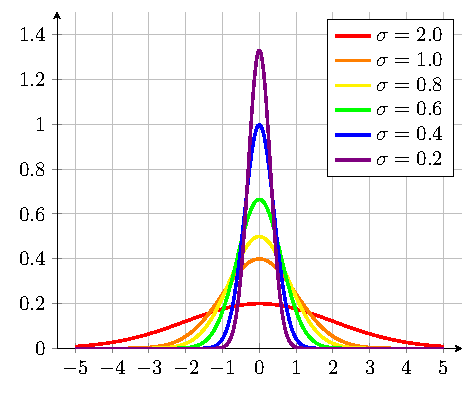
\includegraphics[width=0.5\textwidth]{normal_distributions_different_sigma}\\
		Normal distribution with $\mu=0$ and different $\sigma$s
		\end{multicols}
		
		\begin{multicols}{2}
		\centering
		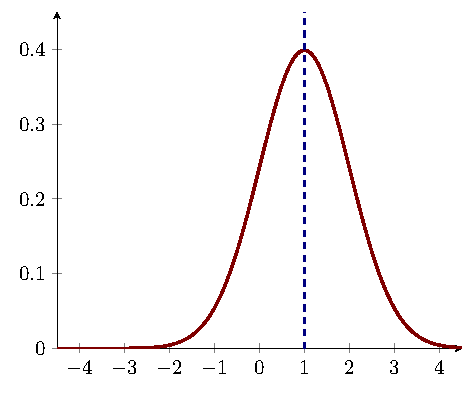
\includegraphics[width=0.5\textwidth]{normal_1-1_density}\\
		Normal density function\\ with $\mu=1$ and $\sigma=1$
		\columnbreak
		
		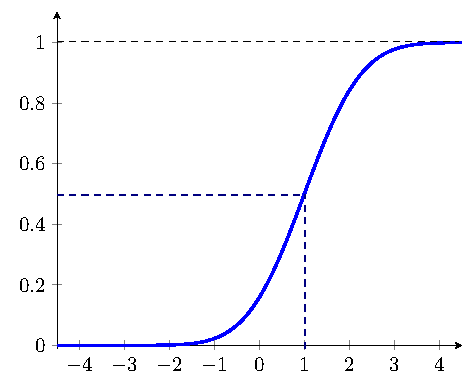
\includegraphics[width=0.5\textwidth]{normal_1-1_CDF}\\
		Normal cumulative distribution function\\ with $\mu=1$ and $\sigma=1$
		\end{multicols}
		
		\begin{multicols}{2}
		\centering
		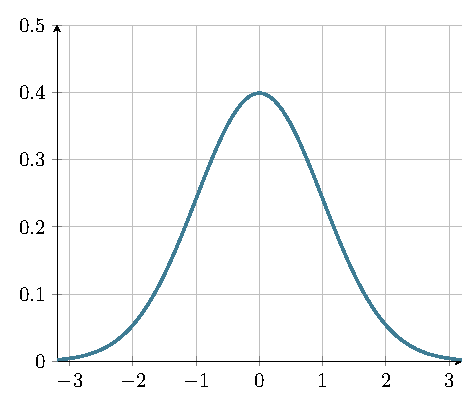
\includegraphics[width=0.5\textwidth]{normal_standard}\\
		Standard normal density function

		\columnbreak		
		
		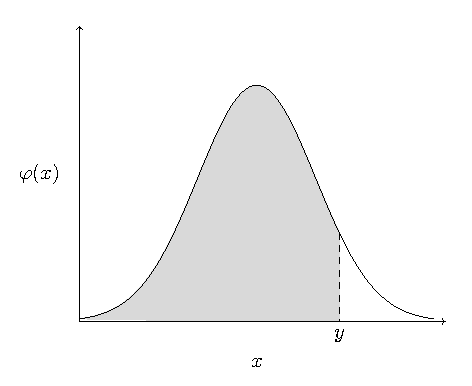
\includegraphics[width=0.5\textwidth]{normal_standard_gray}\\
		Standard normal density function\\ with shaded area at $y$
		
		\end{multicols}


	\subsection{Exponential distribution}
		\begin{multicols}{2}
		\centering
		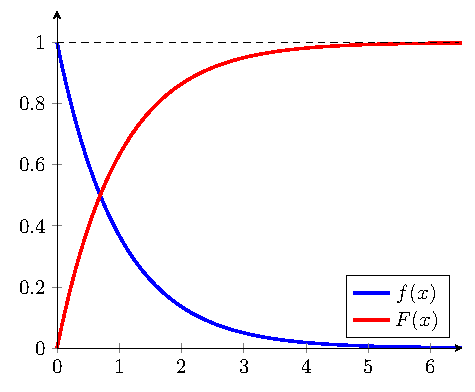
\includegraphics[width=0.5\textwidth]{Exponential_distribution}
		\\
		Exponential distribution, $\lambda=1$\\ density function and cumulative distribution function
		\columnbreak
			
		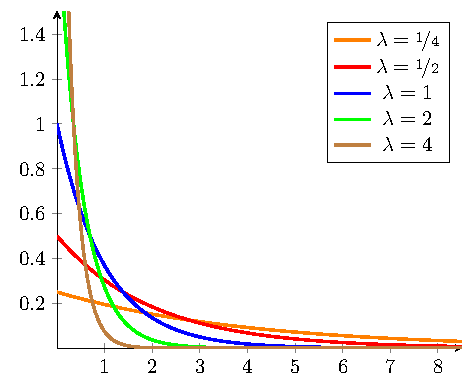
\includegraphics[width=0.5\textwidth]{Exponential_distribution_multiple}
		Exponential distributions\\ with only density functions and different $\lambda$
		\end{multicols}		
\end{document}
